\documentclass[border=10pt]{standalone}

\usepackage{tikz}
\usepackage{tikzsymbols}
\usetikzlibrary{calc,patterns,shapes.geometric}

\def\centerarc[#1](#2)(#3:#4:#5){\draw[#1] ($(#2)+({#5*cos(#3)},{#5*sin(#3)})$) arc (#3:#4:#5);}

\begin{document}
	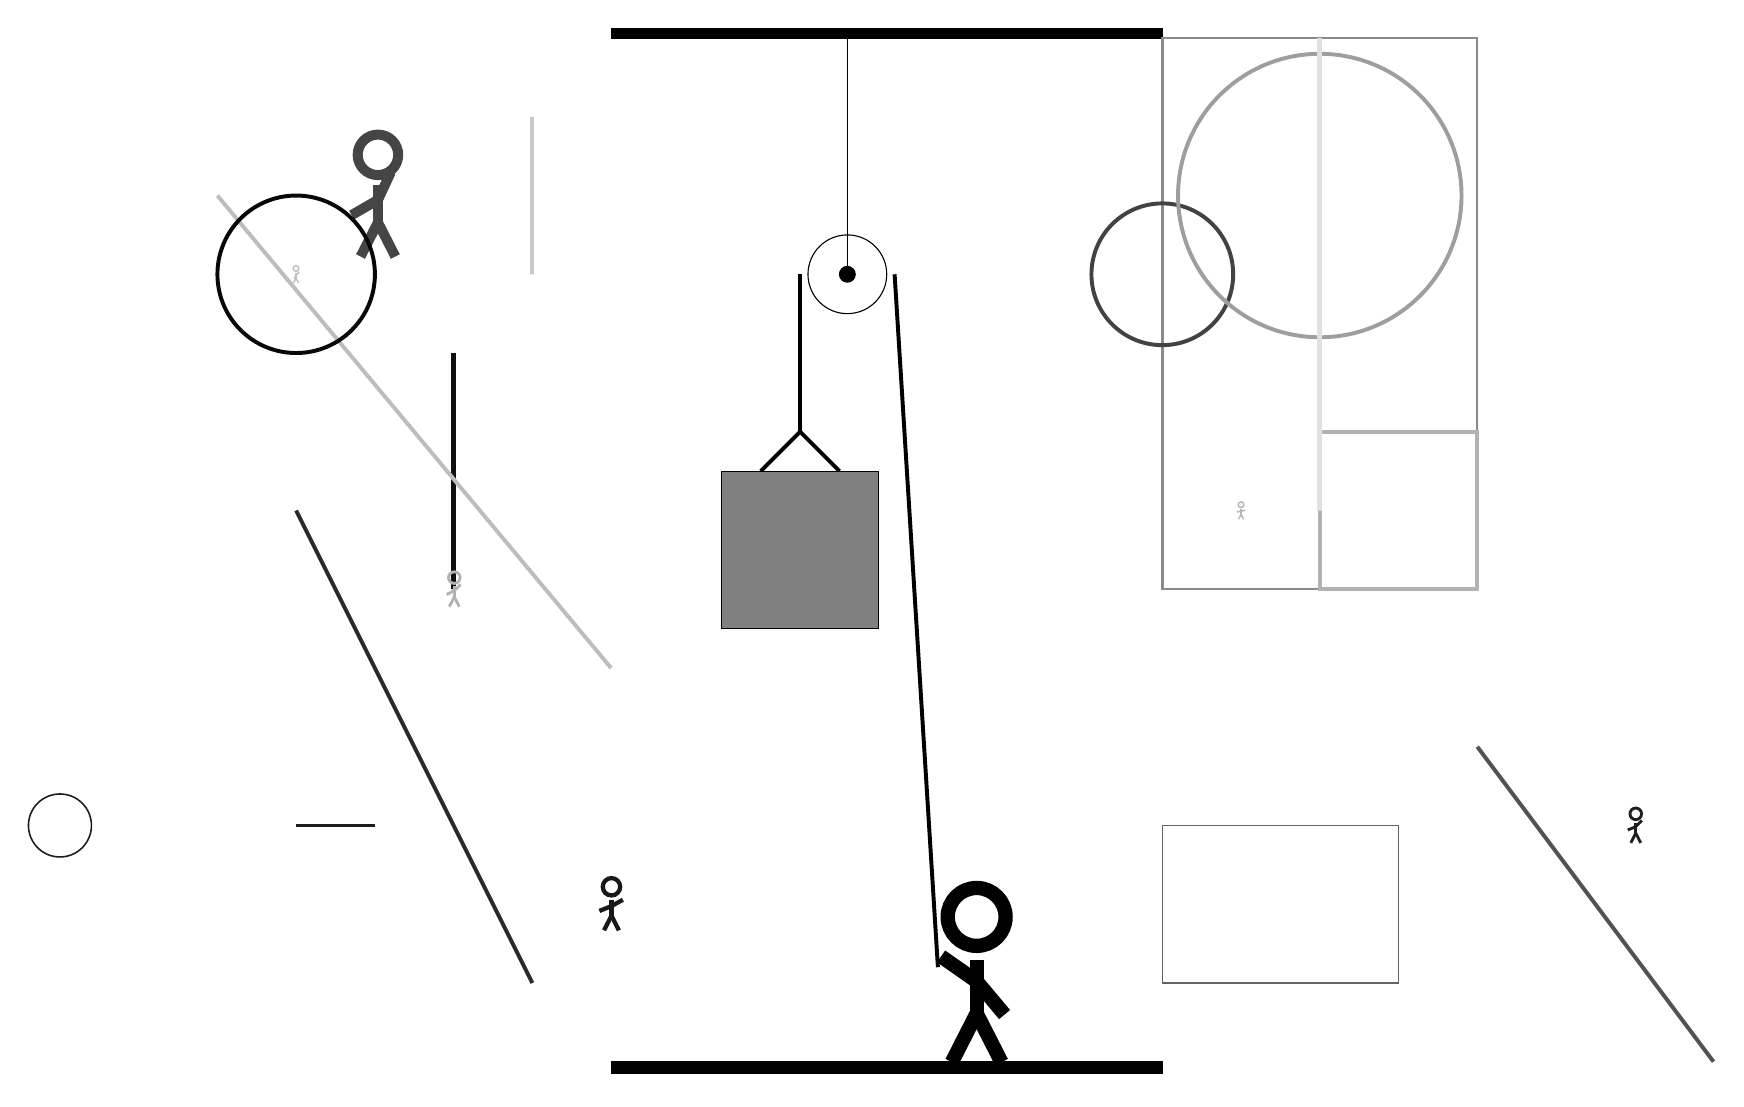
\begin{tikzpicture}
		%%%%% START %%%%%
		
		\draw[fill=black] (-2, 10) rectangle (5, 10.125);
		
		\draw[line width=0.7mm, color=black!94] (-4, 6) rectangle (-4, 3);
		
		\draw [line width=0.4mm, color=black!95](9, -1) circle (0.0);
		\draw[line width=0.3mm, color=black!46] (5, 3) rectangle (9, 10);
		\node[line width=0.6mm, color=black!73] at (-5, 8) {\Strichmaxerl[7][30][65]};
		\draw[line width=0.2mm, color=black!61] (5, 0) rectangle (8, -2);
		\draw[line width=0.5mm, color=black!21] (-3, 9) rectangle (-3, 7);
		
		\node[line width=0.3mm, color=black!90] at (-2, -1) {\Strichmaxerl[3][22][29]};
		\draw[line width=0.5mm, color=black!26](-7, 8) -- (-2, 2);
		\node[line width=0.5mm, color=black!25] at (-6, 7) {\Strichmaxerl[1][66][42]};
		\node[line width=0.3mm, color=black!88] at (11, 0) {\Strichmaxerl[2][22][46]};
		
		\draw [line width=0.5mm, color=black!97](-6, 7) circle (1.0);
		
		\draw[line width=0.5mm, color=black!30] (7, 3) rectangle (9, 5);
		\draw [line width=0.5mm, color=black!63](-5, 3) circle (0.0);
		\draw[line width=0.5mm, color=black!84](-3, -2) -- (-6, 4);
		\draw[line width=0.5mm, color=black!80](-7, 0) -- (-7, 0);
		\draw[line width=0.5mm, color=black!68](9, 1) -- (12, -3);
		
		\draw [line width=0.5mm, color=black!74](5, 7) circle (0.9);
		
		\draw[line width=0.5mm, color=black!89](-5, 0) -- (-6, 0);
		\node[line width=0.4mm, color=black!29] at (6, 4) {\Strichmaxerl[1][12][12]};
		\draw [line width=0.2mm, color=black!89](-9, 0) circle (0.4);
		\draw [line width=0.5mm, color=black!38](7, 8) circle (1.8);
		
		\node[line width=0.3mm, color=black!30] at (-4, 3) {\Strichmaxerl[2][28][43]};
		
		\draw[line width=0.6mm, color=black!12] (7, 4) rectangle (7, 10);
		
		\draw (1, 7) circle (0.5);
		\draw[fill=black] (1, 7) circle (0.1);
		\draw (1, 10) -- (1, 7);
		
		\draw[line width=0.5mm] (-0.1, 4.5) -- (0.4, 5.0) -- (0.9, 4.5);
		\draw[fill=black!50] (-0.6, 4.5) rectangle (1.4, 2.5);
		
		\draw[line width=0.5mm] (0.4, 7) -- (0.4, 5.0);
		\centerarc[line width=0.5mm](1, 7)(0:180:0.6);
		\draw[line width=0.5mm](1.6, 7) -- (2.15, -1.8);
		
		\node at (2.6, -1.9) {\Strichmaxerl[10][-35][-50]};
		
		\draw[fill=black] (-2, -3) rectangle (5, -3.15);
		
		%%%%% END %%%%%
	\end{tikzpicture}
\end{document}